
\item In the circuit shown in the figure, there are two parallel plate capacitors each of capacitance $C$. The switch $S_1$ is pressed first to fully charge the capacitor $C_1$ and then released. The switch $S_2$ is then pressed to charge the capacitor $C_2$. After some time, $S_2$ is released and then $S_3$ is pressed. After some time,
\begin{center}
    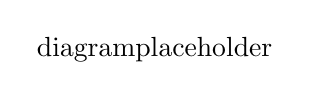
\begin{tikzpicture}
        \node at (0, 0) {diagramplaceholder}; % Replace with actual path to the diagram image if available
    \end{tikzpicture}
\end{center}
\begin{tasks}(2)
    \task the charge on the upper plate of $C_1$ is $2CV_0$.
    \task the charge on the upper plate of $C_1$ is $CV_0$.
    \task the charge on the upper plate of $C_2$ is 0.
    \task the charge on the upper plate of $C_2$ is $-CV_0$.
\end{tasks}
